%==============================================
\subsection{Pushing Mode Generation and Evaluation}\label{subsec:push}
For a selected frontier gap~$g$, this subsection constructs a set of candidate
pushing strategies
$\Xi_g \triangleq \{(\Omega_m,\mathbf{v},\boldsymbol{\xi})\}$,
where~$\mathbf{v} \triangleq (v_x,v_y,\omega)\in\mathbb{R}^3$ is a
short-horizon pushing direction for the movable obstacle~$\Omega_m$ induced by~$g$, and
$\boldsymbol{\xi}\triangleq(\mathbf{c}_m,\mathbf{u})$ is the associated pushing
mode in~\eqref{eq:transition}.
\change{The wrench feasibility encoded in~$\boldsymbol{\xi}$ acts as a screening
condition rather than a force setpoint: it certifies that the chosen contact
configuration can realize the required object motion within the robots'
actuation limits, after which the candidate is passed to the physics rollout for
validation.}



%==============================================
\subsubsection{Direct and Recursive Pushing Tasks}
For \emph{direct push}, let~$\Omega_m$ denote one of the two movable obstacles adjacent to~$g$. For
each such obstacle, a small set of candidate body velocities
$\{\mathbf{v}_m^k\}_{k=1}^{K_m}$ is sampled with a bias toward enlarging the
gap~$g$, while a few angular components are included to account for local
geometry. If the swept region of a direct push intersects movable blockers,
\emph{recursive push} tasks are required instead: for each out-layer
blocker~$\Omega_m$, the nominal direction moves it away from both the swept
region and the reference gap sequence~$\Pi^\star(g)$. Recursion therefore
creates a bounded dependency chain which prioritizes the final
blocker~$\Omega_m$, as shown in Fig.~\ref{fig:direct_recursive_push}.






%==============================================
% \subsubsection{Pushing Mode Generation}
% For each sampled direction~$\mathbf{v}_m^k$ and obstacle~$\Omega_m$, the
% quality of a candidate mode is measured in the body frame. Let
% $\mathbf{v}_m^{k,\mathrm{B}} \in \mathbb{R}^3$ denote~$\mathbf{v}_m^k$
% expressed in the body frame of~$\Omega_m$. For a mode~$\boldsymbol{\xi}$,
% define the primary and multi-directional feasibility losses by:
% \begin{equation}\label{eq:mode-feasibility}
% \begin{aligned}
%   \mathrm{J}_{\texttt{F}}^m
%   (\boldsymbol{\xi},\mathbf{v}_m^{k,\mathrm{B}})
%   &\triangleq
%   \underset{\mathbf{q}_{m,\boldsymbol{\xi}} \in
%   \mathrm{Q}_{m,\boldsymbol{\xi}}}{\textbf{min}}
%   \left\|
%   \mathbf{q}_{m,\boldsymbol{\xi}} +
%   Q_\mu^m(\mathbf{v}_m^{k,\mathrm{B}})
%   \right\|_1,\\
%   \mathrm{J}_{\texttt{MF}}^m
%   (\boldsymbol{\xi},\mathbf{v}_m^{k,\mathrm{B}})
%   &\triangleq
%   \sum_{\mathbf{v}_d \in \mathcal{D}} w_d \cdot
%   \mathrm{J}_{\texttt{F}}^m(\boldsymbol{\xi},\mathbf{v}_d);
% \end{aligned}
% \end{equation}
% where~$\mathbf{q}_{m,\boldsymbol{\xi}} \in \mathbb{R}^3$ is the generalized
% body wrench induced by mode~$\boldsymbol{\xi}$;
% $\mathrm{Q}_{m,\boldsymbol{\xi}} \subseteq \mathbb{R}^3$ is the corresponding
% set of admissible body wrenches under the contact and friction constraints;
% $Q_\mu^m(\mathbf{v}_m^{k,\mathrm{B}}) \in \mathbb{R}^3$ denotes the
% quasi-static friction wrench of~$\Omega_m$ at direction~$\mathbf{v}_m^{k,\mathrm{B}}$;
% $\mathcal{D} \subset \mathbb{R}^3$ is a finite
% set of basis velocities containing the desired direction;
% and~$w_d > 0$ is the
% weight associated with~$\mathbf{v}_d \in \mathcal{D}$. Thus,
% small~$\mathrm{J}_{\texttt{F}}^m(\boldsymbol{\xi},\mathbf{v}_m^{k,\mathrm{B}})$ is
% necessary for force feasibility, while small
% $\mathrm{J}_{\texttt{MF}}^m$ indicates a robust mode.
% Accordingly, the associated mode
% $\boldsymbol{\xi}_m^k \triangleq (\mathbf{c}_m^k,\mathbf{u}_m^k)$ is generated
% by sparse optimization over the reachable part of~$\partial\Omega_m$. The
% reachable boundary is discretized into candidate contacts, and a sparse linear
% program (LP) is solved to minimize
% $\mathrm{J}_{\texttt{MF}}^m(\boldsymbol{\xi},\mathbf{v}_m^{k,\mathrm{B}})$
% under the local friction and wrench constraints.
% Detailed derivations are omitted here for brevity,
% and referred to~\cite{tang2024collaborative,tang2025pushingbots}.
% The resulting nonzero contacts provide~$\mathbf{c}_m^k$, and the corresponding forces
% yield~$\mathbf{u}_m^k$. Only the best few
% pairs~$(\mathbf{v}_m^k,\boldsymbol{\xi}_m^k)$ are retained and collected
% into~$\Xi_g$.

\subsubsection{Pushing Mode Generation}
At a search state~$\mathbf{s}$, a pushing mode is generated for each candidate
direction~$\mathbf{v}_m^k$ and obstacle~$\Omega_m$. In this subsubsection,
contact tuples, object velocities, forces, and wrenches are expressed in the
body frame of~$\Omega_m$. For a contact tuple~$\mathbf{c}$, its
multi-directional force feasibility is:
\begin{equation}\label{eq:mode-feasibility}
\mathrm{J}_{\texttt{MF}}^m(\mathbf{c},\mathbf{v}_m^k)
\triangleq
\sum_{\mathbf{v}_d\in\mathcal{D}_m^k} w_d
\underset{\mathbf{u}\in{U}_m(\mathbf{c})}{\textbf{min}}
\|
\mathbf{q}_m(\mathbf{c},\mathbf{u})
+\mathbf{q}_m^\mu(\mathbf{v}_d)
\| ,
\end{equation}
where~$\|\cdot\|$ is a weighted $\ell_1$ wrench norm, the finite set
$\mathcal{D}_m^k$ perturbs~$\mathbf{v}_m^k$, and
$\mathbf{q}_m^\mu(\mathbf{v}_d)$ is the quasi-static friction wrench; the inner
minimization is a small LP over the admissible forces ${U}_m(\mathbf{c})$.
A state- and direction-dependent contact set
$\mathcal{A}_m^k(\mathbf{s})\subset\partial\Omega_m$ is drawn from the
robot-reachable boundary of~$\Omega_m$ by velocity--force compatibility
filtering (Fig.~\ref{fig:mode_generation}), keeping a contact only if its
robots reach collision-free pre-contact poses. Starting from cached layouts or
random initializations, the tuple is refined by sequential greedy replacement:
at the $\ell$-th step, $\mathbf{c}_{r,c}^{\ell}$ replaces the $r$-th contact
with $c$, and the best replacement is:
\begin{equation}
c^\star
=
\underset{c\in\mathcal{A}_m^k(\mathbf{s})}{\textbf{argmin}}\;
\mathrm{J}_{\texttt{MF}}^m
\bigl(\mathbf{c}_{r,c}^{\ell},\mathbf{v}_m^k\bigr),
\label{eq:greedy_mode_update}
\end{equation}
swept over contact slots until $\mathrm{J}_{\texttt{MF}}^m$ no longer
decreases; a bounded backtracking variant removes the robot-order sensitivity
of this replacement. If no full-team assignment exists for a task, e.g., on
small faces or under the pairwise pusher-clearance constraint, one robot is
released for that single push (charged a penalty when ranking modes, so
full-team modes are preferred) and the full team is available again afterwards.
The best tuple over initializations gives
$\mathbf{c}_m^{k,\star}$, from which $\mathbf{u}_m^k$ follows from the inner
minimization in~\eqref{eq:mode-feasibility}, yielding
$\boldsymbol{\xi}_m^k=(\mathbf{c}_m^{k,\star},\mathbf{u}_m^k)$; each mode is
cached as a warm start. The best few admissible pairs are kept for gap~$g$ and
passed to simulation; $\mathbf{u}_m^k$ certifies wrench feasibility while
hardware tracks the contact geometry from pose/velocity commands.

% The best refined mode over all initializations is denoted by
% $\boldsymbol{\xi}_m^k=(\mathbf{c}_m^k,\mathbf{u}_m^k)$.
% It is admitted only if its rollout is validated in simulation.
% Accepted modes are stored in a persistent \textsc{mode-cache},
% indexed by discretized shape, mass, available robot force, and pushing direction,
% and reused as warm starts.
%------------------------------
\begin{figure}[t!]
  \centering
  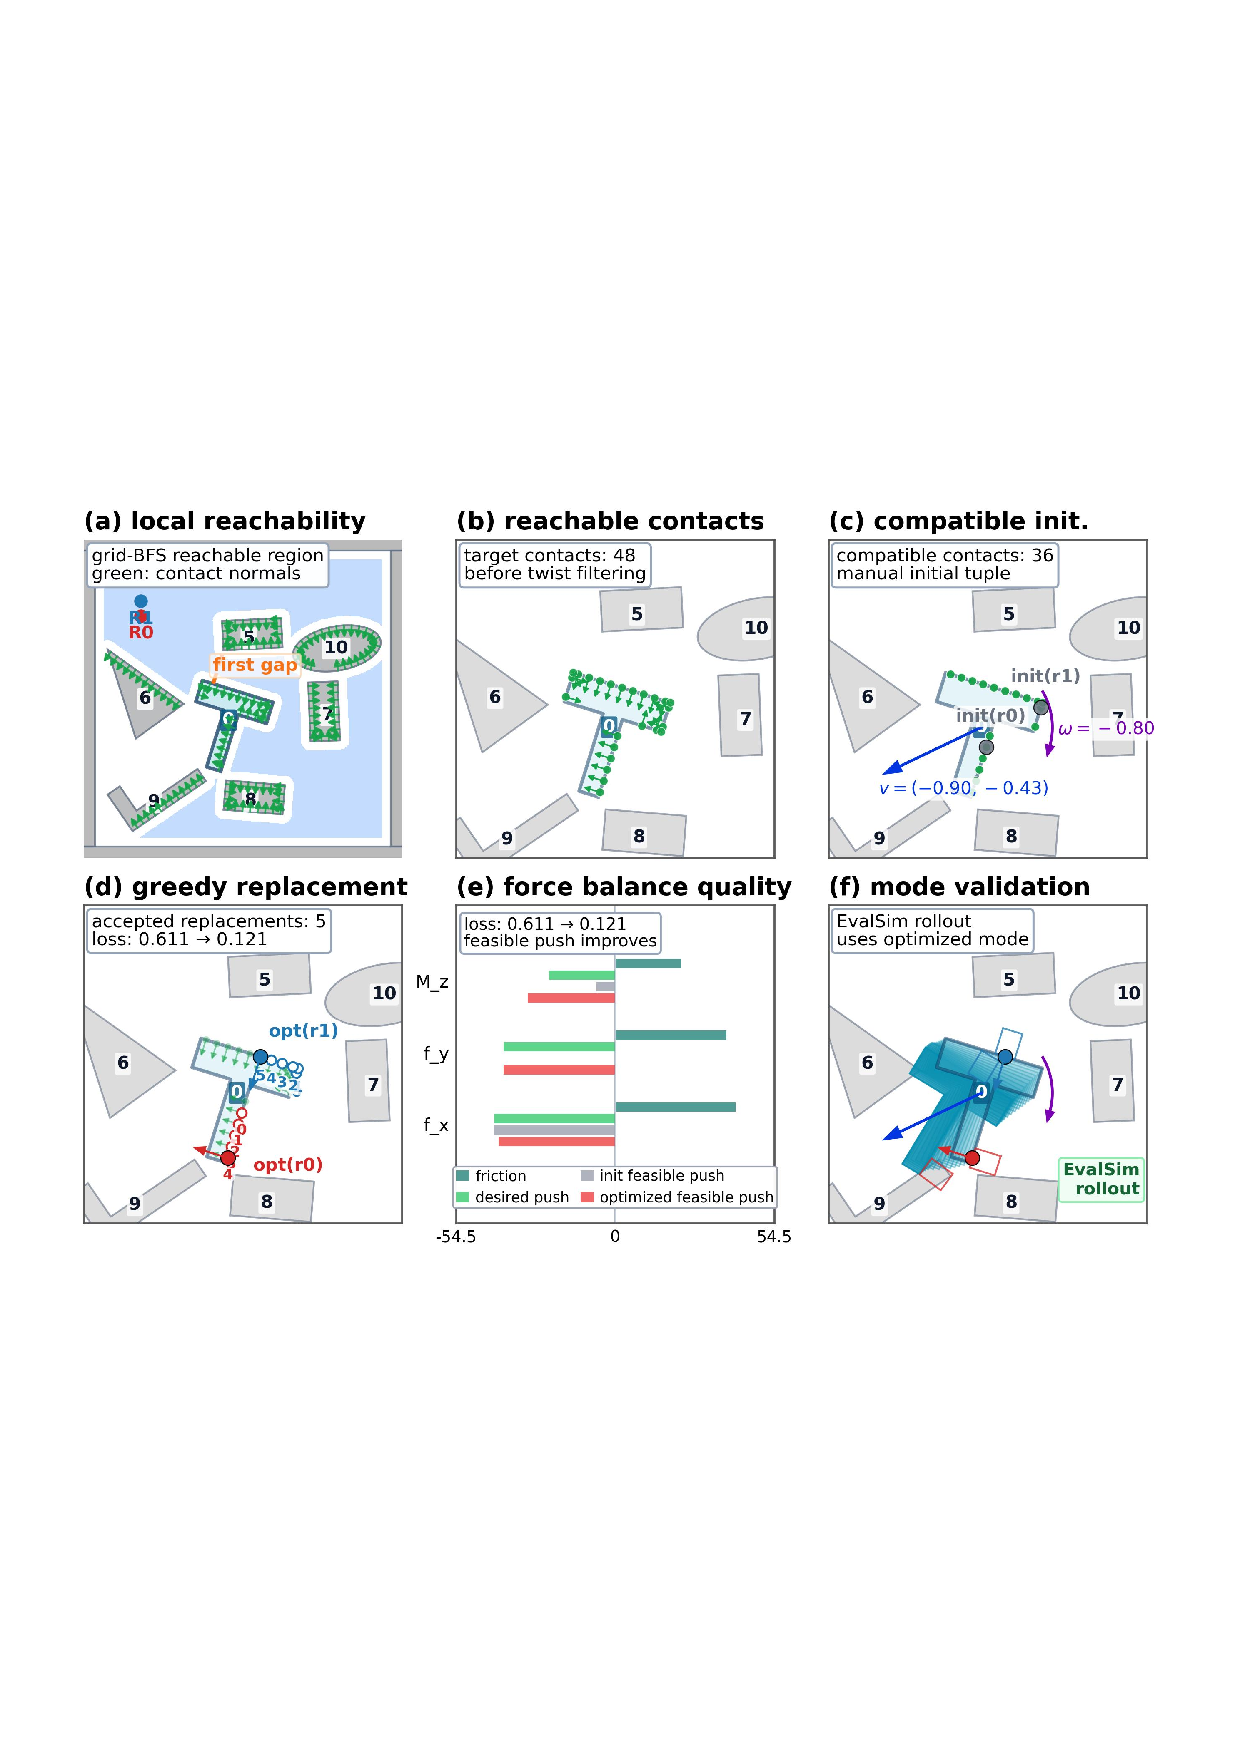
\includegraphics[width=0.8\linewidth]{figures/mode_generation.pdf}
  \vspace{-4mm}
  \caption{\change{
Reachable contacts are filtered by the
  desired object twist, assigned to robots, refined by local replacement,
  and finally validated by simulation.}}
    \label{fig:mode_generation}
   \vspace{-4mm}
\end{figure}
%------------------------------
%==============================================
\subsubsection{Pushing Strategy Evaluation}

For a current state~$\mathbf{s}$ and a candidate strategy
$(\Omega_m,\mathbf{v},\boldsymbol{\xi})\in\Xi_g$, a short-horizon rollout
evaluates the transition in~\eqref{eq:transition} under the selected mode.
As shown in Fig.~\ref{fig:mode_generation}, a strategy is accepted only if
the robots reach the pre-contact poses, maintain stable contact, and induce
obstacle motion above threshold. The simulation returns:
\begin{equation}
    (\mathbf{s}',\,\delta_{\texttt{T}},\,\delta_{\texttt{J}})
    \triangleq
    \mathsf{EvalSim}
    \big(
    \mathbf{s},(\Omega_m,\mathbf{v},\boldsymbol{\xi})
    \big),
    \label{eq:sim}
\end{equation}
where~$\mathbf{s}'$ is the successor state capturing the resulting robot and
object configurations; $\delta_{\texttt{T}}>0$ is the time cost; and
$\delta_{\texttt{J}}$ is the control effort. 
\change{
The rollout jointly simulates
all robots and movable bodies, thereby capturing contact-induced object
interactions.}
For efficiency, the pushing rollout may be bypassed when the mode has been
validated before and the swept region of~$\Omega_m$ is collision-free.
%------------------------------
\begin{figure}[t!]
  \centering
  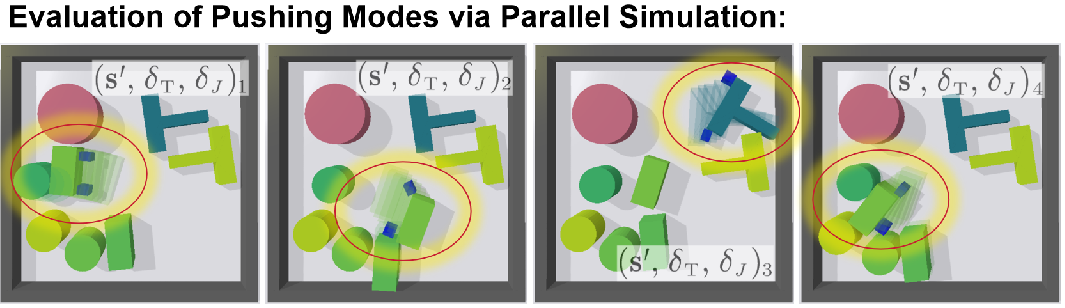
\includegraphics[width=0.8\linewidth]{figures/PIHS_bottom.pdf}
  \vspace{-2mm}
  \caption{\change{Sampled push tasks are evaluated via parallel simulation,
  producing updated states for search expansion.}}
    \label{fig:PIHS}
   \vspace{-4mm}
\end{figure}
%------------------------------
